\usetikzlibrary{arrows.meta}
% id: 1994_old_subject_science_q24_fig1; family: basic_conic
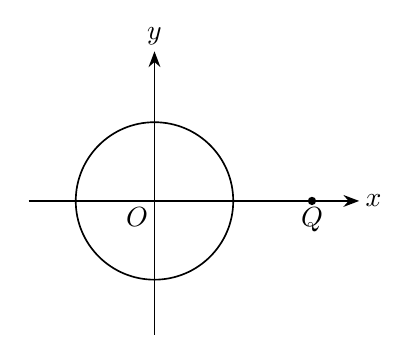
\begin{tikzpicture}[x=1cm,y=1cm,line width=.6pt,font=\normalsize,every node/.style={inner sep=0pt},>=Stealth]
\draw[->] (-1.6,0)--(2.6,0) node[right,inner sep=0pt,xshift=2pt] {$x$};
\draw[->] (0,-1.7)--(0,1.9) node[above,inner sep=0pt,yshift=2pt] {$y$};
\draw (0,0) circle[radius=1cm];
\fill (2,0) circle[radius=1.5pt];
\node[anchor=north east,inner sep=0pt,xshift=-2pt,yshift=-2pt] at (0,0) {$O$};
\node[anchor=north,inner sep=0pt,yshift=-2pt] at (2,0) {$Q$};
\end{tikzpicture}
